\documentclass[11pt]{article}

\usepackage[paper=a4paper,margin=0.75in]{geometry}
\usepackage{setspace}
\usepackage{amsmath,amsfonts,amssymb,amsthm}
\usepackage{graphicx}
\usepackage{hyperref, xcolor}
\usepackage{mathrsfs}
\usepackage{bm, bbm}
\usepackage[bottom]{footmisc}
{
	\newtheorem{assumption}{\textit{Assumption}}
	\newtheorem{definition}{\textit{Definition}}
	\newtheorem{theorem}{\textit{Theorem}}
}
\usepackage{fancyhdr}
\pagestyle{fancy}
\rhead{\today}
\lhead{Industrial Organisation Revision -- Lecture 5}
\numberwithin{equation}{section}

\newcommand\blfootnote[1]{%
	\begingroup
	\renewcommand\thefootnote{}\footnote{#1}%
	\addtocounter{footnote}{-1}%
	\endgroup
}

\begin{document}
\onehalfspacing

\section{A Canonical Insurance Model: Notation}
\blfootnote{These notes are based on Howard Smith's lectures from the 2018-2019 academic year.\\
Of course, this is our interpretation of the material Howard presented. Good content is his; mistakes are ours.}

\vspace{-1cm}
\begin{itemize}
 \item Agents are each characterised by a vector $\zeta = (\textbf{x}, \nu)$, where $\nu$ is unobservable to firms;
 \item $\phi$ is the vector of insurance characteristics (e.g. what is covered and by how much);
 \item $p$ is the price of the contract;
 \item $S$ is the set of possible future scenarios for the agent, $s \in S$.
\end{itemize}
Agents are assumed to have \textbf{quasi-linear utility} in prices (no income effects)
\begin{equation}
	\label{agentutility}
	u(s, \zeta, \phi) - p
\end{equation}
they're also assumed to value contracts by their \textbf{expected utility} which, defining probabilities as $\pi(\cdot)$, is
\begin{equation}
	\label{eu}
	v(\phi, \zeta) = \sum_{s \in S} \pi(s|\zeta)u(s, \zeta, \phi)
\end{equation}
The expected outcome for a consumer characterised by vector $\zeta$ is
\begin{equation}
	s(\zeta) = \sum_{s \in S} \pi(s|\zeta)s
\end{equation}
To the insurer, the cost of agent's outcome $s$ under contract $\phi$ is $\tau(s,\phi)$. This cost is observable; thus the expected cost of serving an agent is
\begin{equation}
	\label{cost}
	c(\phi, \zeta) = \sum_{s \in S} \pi(s|\zeta) \tau(s, \phi)
\end{equation}
and aggregate welfare is given by (since price is a zero-sum transfer)
\begin{equation}
\label{welfare}
	W = \int v\big( \phi(\zeta), \zeta \big) - c\big( \phi(\zeta), \zeta \big)~ dG(\zeta)
\end{equation}

Consumer $i \in I$ chooses contract $j \in J$ iff $v(\phi_j, \zeta_i) - p_j \geq v(\phi_k, \zeta_i)
 - p_k, ~\forall~ k \in J$; let $I(j) \subseteq I$ be the set of such agents.

 Differences in \textbf{(i)} contract unit \textbf{costs} to the insurer and \textbf{(ii)} rates of \textbf{incidence} of outcomes $s$ arise due to the irrepresentativeness of the population sample that selects into each contract $j$ (\textit{self-selection}). \\
 These are not necessarily the consequences of asymmetric information, as they could result from differences in \textbf{x}; however, if differences persist \textit{after} conditioning on the set of characteristics observable to the insurer, selection might be the reason: that is,
\begin{equation}
\label{infasym}
	\mathbb{E}_x[s|i \in I(j); x_i = x] \neq \mathbb{E}_x[s|i \in I(k); x_i = x]
\end{equation}
 is supportive of informational asymmetries between insurers and agents. Note however that asymmetric information generates two underlying effects that contribute to the difference above: \eqref{infasym} can be rewritten as
  	\begin{equation}
 \label{decomposition}
	\begin{split}
 	\mathbb{E}_x[s|i \in I(j);\phi_j; x_i = x] - \mathbb{E}_x[s|i \in I(k);\phi_k; x_i = x] = \\ \color{red}{\mathbb{E}_x[s|i \in I(j);\phi_j; x_i = x] - \mathbb{E}_x[s|i \in I(k);\phi_j; x_i = x]} ~\color{black}{+} \\ \color{blue} {\mathbb{E}_x[s|i \in I(k);\phi_j; x_i = x] - \mathbb{E}_x[s|i \in I(k);\phi_k; x_i = x]}
	\end{split}
 \end{equation}
  where the second line expresses a \textbf{selection effect} resulting from the agents \textit{being different} conditional on their contract choice, while the third line expresses the \textbf{incentive effect} from having different contracts. Simple tests of asymmetric information will not distinguish between the two.

  \section{Chiappori and Salani\'{e} (2000)}

Analysis of the French car insurance market. Two most common insurance contracts: Low (L, minimum coverage) and High (H, covers more damages).

The authors propose two tests of asymmetric information: a parametric test relying on a pair of probits (or, more efficiently, a bivariate probit); and a non-parametric test relying on a $\chi^2$ test of independence.

\subsection{Pair of Probits / Bivariate Probit}

For each individual $i = 1,\dots, N$, we have exogenous variables $X_i$ and two endogenous dichotomous variables: \textbf{(i)} whether has purchased H insurance, and \textbf{(ii)} whether has caused any accident. The two endogenous variables have the following probit specification
\begin{equation}
H_i = \mathbbm{1} \{X_i \beta + \epsilon > 0\} \hspace{2cm} acc_i = \mathbbm{1} \{X_i \gamma + \eta > 0\}
\end{equation}
where by assumption the unobserved components
\[
\begin{bmatrix}
\epsilon \\
\eta
\end{bmatrix}
\sim N \bigg(
\begin{bmatrix}
0 \\ 0
\end{bmatrix}
,
\begin{bmatrix}
1 & \rho \\
\rho & 1
\end{bmatrix}
\bigg)\]
For the $\rho = 0$ case, the equations can be separately estimated and generalised residuals obtained as
\begin{equation}
	\hat{\epsilon_i} = \frac{\phi(X_i \hat{\beta})}{\Phi (X_i \hat{\beta})}y_i - (1 - y_i) \frac{\phi(X_i\hat{\beta})}{\Phi(-X_i \hat{\beta})} \hspace{2cm}
	\hat{\eta_i} = \frac{\phi(X_i \hat{\gamma})}{\Phi (X_i \hat{\gamma})}y_i - (1 - y_i) \frac{\phi(X_i\hat{\gamma})}{\Phi(-X_i \hat{\gamma})}
\end{equation}
A test statistic can then be formed, under the null of conditional independence $cov(\epsilon_i, \eta_i) = 0$, as
\begin{equation}
	\Omega = \frac{(\sum_i \hat{\epsilon_i}\hat{\eta_i})^2}{\sum_i \hat{\epsilon_i}^2\hat{\eta_i}^2} \sim \chi^2(1)
\end{equation}
If $\rho = 0$ is not assumed, it is more efficient to estimate the bivariate probit system: a Wald test of the $\rho = 0$ null is then a valid test of independence given the assumed normality of error terms.

\subsection{Non-Parametric Test}

This test is based on the popular $\chi^2$ test of independence. First, transform $X_i$ in $m$ dummy variables; this effectively creates $2^m$ cells, in each of which all individuals share all characteristics. For each cell, create a two-by-two table classifying agents based on their values of the two dichotomous endogenous variables; then, defining $Z_{H,acc}$ as the number of agents within each cell with $H = \{0,1\}$ and $acc = \{0,1\}$, and $Z$ as the total number of agents in the cell, define the test statistic
\begin{equation}
  T = \sum_{H, acc = \{0,1\}} \frac{\big[Z_{H, acc} - \big(Z_H Z_{acc} / Z\big) \big]^2}{Z_{H, acc}}
\end{equation}
which, under within-cell (i.e. conditional) independence of $H$ and $acc$, is $\chi^2$-distributed. There are $2^m$ such statistics: their sum is distributed, under conditional independence, as $\chi^2 (2^m)$.\footnote{Alternatives include the Kolmogorov-Smirnov test for the empirical CDF of test statistics and a binomial distribution test that relies on a sharp arbitrary threshold.}

\subsection{Empirical Results}
None of the aforementioned tests can, somewhat surprisingly (?), reject conditional independence of the endogenous variables. At least for some parts of the driver population there seems to be no evidence of abused asymmetric information. It should be noted that all of these tests are tests of \textit{presence} of asymmetric information, binary in their nature:\footnote{Also, they cannot distinguish between adverse selection and moral hazard.} they say nothing about the welfare implications of the market failure. For that, we need to impose further structure on the problem.

\section{Einav, Finkelstein and Cullen (2010)}
\subsection{Setting Sketch}
Assume a competitive insurance market in which all firms offer two contracts $\phi = \{H,L\}$ at prices $p_L = 0; ~p_H=p$. Consumer utility from the $L$ contract is normalised to zero; as a result, $H$ is chosen whenever $v(H, \zeta_i) - p > 0$. Aggregate demand is
\begin{equation}
	Q(p) = \int \mathbbm{1}\{v(H, \zeta) - p > 0\} ~d G(\zeta)
\end{equation}
and inverse demand is $P(Q) \equiv Q^{-1}(Q)$. Average cost then is
\begin{equation}
\begin{split}
AC(p) = \frac{1}{Q(p)} \int c(H, \zeta_i) \mathbbm{1}\{v(H, \zeta) - p > 0\} ~d G(\zeta) = \\ = \mathbb{E}_\zeta [c(H, \zeta)| v(H, \zeta) > p]
\end{split}
\end{equation}
and marginal cost is
\begin{equation}
MC(p) = \mathbb{E}_\zeta [c(H, \zeta)| v(H, \zeta) = p]
\end{equation}
As for welfare, \eqref{welfare} can be split in consumer surplus
\begin{equation}
	CS(p) = \int \mathbbm{1}\{v(H, \zeta) - p > 0\}[v(H, \zeta) - p] dG(\zeta)
\end{equation}
and producer surplus
\begin{equation}
PS(p) = \int \mathbbm{1}\{v(H, \zeta) - p > 0\}[p - c(H, \zeta)] dG(\zeta)
\end{equation}
implying that it is socially efficient to ensure agents for whom $v(H, \zeta_i) > c(H,\zeta_i)$. \\

Note that under the perfect competition assumption firms set equal prices for the same contracts so each company gets a random draw from the pool of insurance buyers. Moreover, the `insurance production function' is the same ensuring average costs are the same. Importantly, the equilibrium will be one where $\mathbf{p = AC(p)}$: any higher price would imply 0 demand, any lower price would induce a loss.\footnote{Intuitively, there will be no marginal cost pricing as a result of different agent types: the seller targets an `average' agent to cross-subsidise losses from adversely selected agents with gains from less risky agents.}

Furthermore note that, in this competitive market characterised by adverse selection, \textbf{demand, MC and AC curves are all downward sloping} in the Quantity-Price space.
This is because the first units sold go to those who have the largest valuation, which implies the largest cost to the insurer.
As quantity increases, insurance is sold to less `expensive' agents, and thus firms are going to \textbf{lower} prices (which are kept at no-profit levels by the perfect competition assumption): hence the downward curves.
Clearly, at 0 quantity AC=MC; as quantity increases, \textbf{MC slopes downwards faster than AC} because the latter, being an algebraic mean, is weighed by the larger cost of the early units, while the former is not -- in econspeak, AC includes the burden of cross-subsidising agents due to adverse selection while MC does not, representing the perfect information case.
Asymmetric information implies a deadweight loss which can be depicted as a cute triangle (see below).

\begin{center}
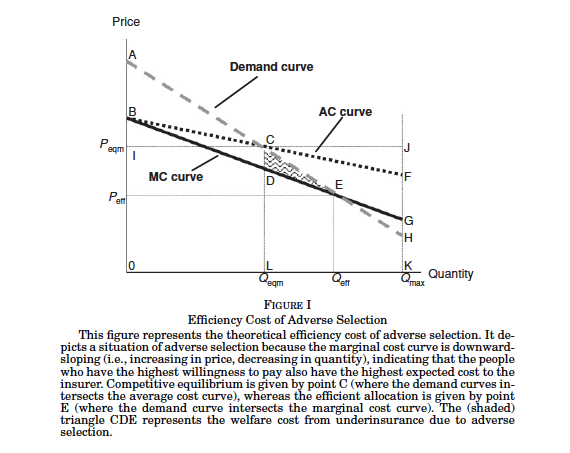
\includegraphics[width=0.75\textwidth]{p1}
\end{center}

However, note that \textbf{advantageous selection} is just as sensible: if risk averse agents see obtaining insurance and taking precautionary actions as complements, those who demand more insurance might actually be the less expensive.
In that case, MC and AC curves would be \textbf{upward} sloping; the market inefficiency would now result from agents buying \textbf{too much} insurance -- as low-risk high-valuation agents will subsidise provision of underpriced contracts to high-risk low-valuation types.
There's a cute picture for this too, in the next page. \\

The idea of Einav, Finkelstein and Cullen is that these \textbf{demand and cost curves are sufficient statistics for welfare analysis} in the pure \textit{Marschak maxim} sense; that is, the curves mediate the information content of the primitives, thus making knowledge of the primitives superfluous once the curves have been estimated.
The authors then ``estimate the demand and cost curves but remain agnostic about the underlying primitives that give rise to them'' (p. 890), as ``the precise \textit{source} of selection is not germane for analysing the efficiency consequences of the resultant selection, or the welfare consequences of public policies that change the equilibrium price'' (\textit{ibidem}).
Of course this requires \textbf{insurance contracts to be predetermined} -- only their prices are allowed to change.

\begin{center}
	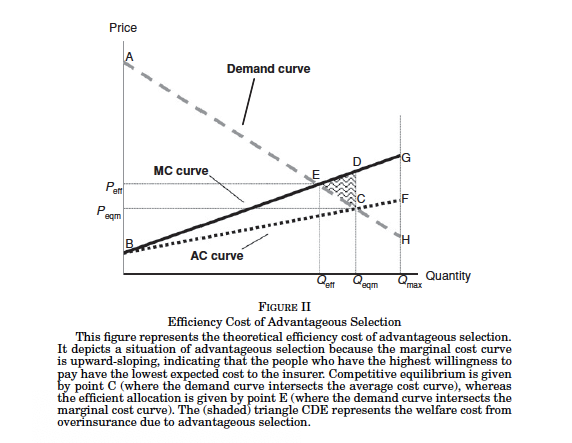
\includegraphics[width=0.75\textwidth]{p2}
\end{center}

\subsection{Empirical Analysis}
Data on health insurance purchases by 3779 Alcoa workers. Two levels of coverage, H and L, detailed demographics (including health conditions, which allows to calculate costs to the insurer). The setting is particular because, within the firm, employees doing comparable jobs in different organisational units face different insurance costs that are quasi-random.

Given price is assumed to be exogenous, the world smiles at the authors: they estimate a linear probability model for $Q_i$, whether $i$ demands high insurance or not, and a linear regression for costs to the insurer
\begin{equation}
	\label{efccrazyeconometrics}
	Q_i = \alpha + \beta p_i + \epsilon_i \hspace{2cm} AC_i = \gamma + \delta p_i + u_i
\end{equation}
note the information from these two curves is sufficient to back out the marginal cost curve: in fact, given aggregate average costs and quantities for each contract,
\begin{equation}
	TC(p) = AC(p)Q(p) \hspace{2cm} MC(p) = \frac{\partial TC(p)}{\partial Q(p)} = \frac{\partial AC(p)Q(p) / \partial p}{\partial Q(p) / \partial p} = \frac{AC(p)\beta + Q(p)\delta}{\beta}
\end{equation}

Estimation by OLS suggests that demand is \textbf{decreasing} in price of H, and that the average cost of agents who select into more costly contracts is higher -- indicating adverse selection. The welfare loss is about 3\% of total estimated surplus; however, this welfare loss is lower than the loss that would be incurred under a mandated high contract. Estimation results are below.

\begin{center}
	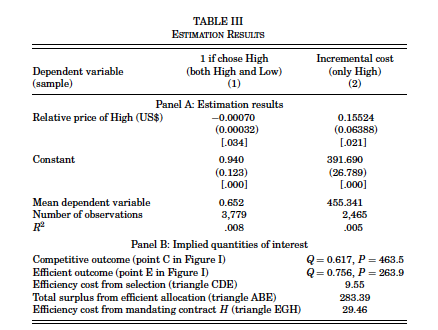
\includegraphics[width=0.75\textwidth]{p3}
\end{center}

\section{Einav, Finkelstein and Schrimpf (2010)}

UK market for annuities: at retirement, people are forced to annuitise accumulated funds in retirement savings accounts.
Individuals are allowed a choice of \textit{guarantee period} between 0, 5, and 10 years, which ensures an annuitised stream \textbf{irrespective of death} for the chosen period.
The longer the guarantee period, however, the smaller the stream returned while alive: no reason to select guarantee shorter than expected life span.

Under perfect competition and complete information, each plan would have a net expected return of 0 for retirees conditional on their type $\zeta_i = (\mathbf{x}_i, \mathbf{\nu}_i)$.
Under imperfect information, there is scope for \textbf{self-selection on likelihood of premature death} as riskier agents select longer guarantees to leave to their dependents.
The authors set to estimate the welfare losses from this selection.

Data on age, guarantee selected, year of death and contract information for 9000+ retirees.

\subsection{Model}

For each consumer, $\mathbf{x}_i = \{sex_i, age_i\}$, $\mathbf{\nu}_i = \{\alpha_i, \beta_i\}$ -- where $\alpha_i$ is heterogeneity in the propensity to die and $\beta_i$ is heterogeneity in taste for bequest.
Agents with large draws of $\alpha$ and $\beta$ will be more likely to select into longer guarantees.

The probability of dying is given by hazard rate $\kappa_t(\alpha_i, \lambda)$, with $\kappa_t'(\alpha_i) > 0$ and $\lambda$ being a shape parameter.
Utility for period $t$ is defined as
\begin{equation}
	v(w_t, c_t) = [1-\kappa_t(\alpha_i, \lambda)]u(c_t) + \kappa_t(\alpha_i, \lambda) \beta_i u(w_t + Z_t^\phi)
\end{equation}
where $c_t$ is consumption, $w_t$ is the value of assets, and $Z^\phi_t$ is the present value of post-death guarantee payments ($\phi \in \{0,5,10\}$).

The optimal consumption plan then obeys
\begin{equation}
	\begin{gathered}
		\label{bellman}
	V^\phi (w_t, \zeta_i) = \max_{c_t \geq 0}[1-\kappa_t(\alpha_i, \lambda)]\{u(c_t) + \delta V^\phi (w_{t+1}, \zeta_i)\} + \kappa_t(\alpha_i, \lambda) \beta_i u(w_t + Z_t^\phi) \\
	s.t. ~~ w_{t+1} = (1+r)(w_t + Z_t^\phi - c_t) \geq 0
		\end{gathered}
\end{equation}
and the choice of guarantee $\phi$ obeys $\max_\phi V^\phi (w_t, \zeta_i)$. \\

The model is estimated with some useful parametric assumptions: first, on the form of the mortality hazard rate; second, imposing CRRA utility; third, assuming that $\{\alpha, \beta\}$ is bivariate lognormal (with unspecified mean, variance and covariance to be estimated). Furthermore, the discount factor $\delta$, the CRRA parameter and the interest rate are calibrated. \\

The log-likelihood for the sample is then relatively easy to derive: the probability of $i$ dying at age $s$ after having chosen guarantee $\phi$ is
\begin{equation}
Pr(s, \phi | \alpha, \lambda) = Pr(s | \phi, \alpha, \lambda ) \times Pr(\phi | \alpha, \lambda )
\end{equation}
denote by $\mu$ and $\Sigma$ the mean vector and variance-covariance matrix for the joint distribution of $\alpha$ and $\beta$; the likelihood then is
\begin{equation}
	\mathscr{L}_i(s, \phi | \mu, \Sigma, \lambda) = \int_\alpha Pr(s | \phi, \alpha, \lambda ) \times Pr(\phi | \alpha, \lambda ) d F(\alpha; \mu, \Sigma)
\end{equation}
and the maximum likelihood estimator is defined as, for $\theta = \{\mu, \Sigma, \lambda\}$,
\begin{equation}
	\hat{\theta} \in \arg \max_\theta \sum_i \ln \mathscr{L}_i(s, \phi | \mu, \Sigma, \lambda)
\end{equation}

Incidentally, the estimation procedure is actually \textit{significantly} more complicated: in the paper, $\lambda$ is first estimated by maximum likelihood; conditional on this estimate, a second maximum likelihood estimator yields distributional parameters of the heterogeneity.
However, the second maximum likelihood estimator requires in principle re-evaluating the decision rule \eqref{bellman} for the continuum of $\alpha$ values.
The computation is simplified by the monotonicity of optimal guarantee choice in the heterogeneity, which allows to (i) define cutoff rules for guarantee choice; (ii) calculate cutoffs \textit{once} for a grid of $\alpha$; (iii) interpolate likelihood. The two-step MLE is necessary for computational feasibility as the second MLE would otherwise require iterating over the $\lambda$ space as well.

\subsection{Results}

The authors find significant heterogeneity in both propensity to die $\alpha$ and taste for bequest $\beta$; furthermore, they find a \textbf{large positive correlation} between the two components.

\begin{center}
	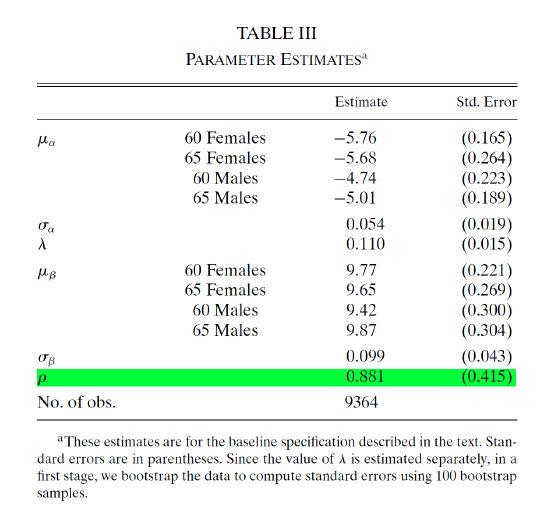
\includegraphics[width=0.6\textwidth]{efs1}
\end{center}

\subsection{Welfare}

To analyse the implications of the model for welfare, the authors use its estimates to compute the `wealth equivalent' for each individual, i.e. the amount of wealth that would make her indifferent with choosing her actual wealth and annuity.
Given an actuarially fair annuity rate and a risk averse individual, the wealth equivalent will be \textbf{higher} than actual wealth plus guarantee, as the guarantee removes the risk from dying.\footnote{If one selects the wealth equivalent, one can only consume it, while the guarantee can be passed to dependents and generate further utility upon death; hence, the wealth equivalent must be larger to induce consumers to accept it.}
However, for an annuity rate sufficiently below the perfect information equilibrium, the wealth equivalent can be \textbf{lower}.
In general, the difference gives an estimate of the consumer gain from the availability of the guarantee: this allows authors to estimate the value of available contracts, as well as counterfactuals -- e.g. with a compulsory guarantee of 10 years, without guarantee, etc. \\

The first finding is that, as expected, the \textbf{main beneficiaries from the pooling equilibrium are low-$\alpha$ individuals}: they enjoy higher annuity rates than required as a result of the effort by companies to deter high-$\alpha$ from selecting into longer guarantees.\footnote{Note also that \textbf{low-$\beta$ individuals} benefit from the annuity market as they care less about not having wealth at death (without the annuity market, they would have to keep their entire wealth non-annuitised at a risk).}
Fixing asymmetric information allows firms to price optimally and transfers the surplus away from these agents, benefitting discriminated-against higher-$\alpha$ agents. \\


A second finding is that the effect of a \textbf{mandated guarantee} largely depends on the length of the mandated contract, and that the optimal choice critically depends on the joint distribution of risk and preferences.
The mandated guarantee length that improves over the status quo the most is a \textbf{mandated 10-year guarantee}; however, by the compulsory nature of the UK system, it is not possible to account for the welfare response of those who \textbf{do not} want to annualise their retirement savings.



\end{document}
